\subsection{Completed External Source-Receiver Study}
\label{sec:sourcecount-complete}
The external source-count matrix is complete: 360 new models and 2520 seven-view readouts, each with 144000 physical packets. It covers $m=1,2,3,4,6$, four methods with their own CE controls, and three model seeds. Natural-budget supervised, natural-budget ordinary PL, and fixed-L/V supervised settings contain 120 models each. The fixed target RX set is $(0,2,5,7,9,10)$; source prefixes follow $(1,3,4,6,8,11)$. The preregistered effective matrix excludes the five-source point. Historical five-source results on seven target RX are not inserted into these curves.

An independent CPU audit recomputed frozen predictions and verified source checkpoints/complete training records. Aggregate recomputation checked 93240 confusion matrices and matched 6440 summary/paired statistics against that audit. All reported cells contain all three seeds. Figure~\ref{fig:sourcecount-accuracy} separates natural supervised/PL from fixed L/V supervision; six-scene means are formed within seed before cross-seed sample SD. Error bars quantify model-seed variation conditional on the same source prefix and target set, not variation over receiver selections. There is no measured $m=5$ point or inferred value.

\begin{figure*}[t]
\centering
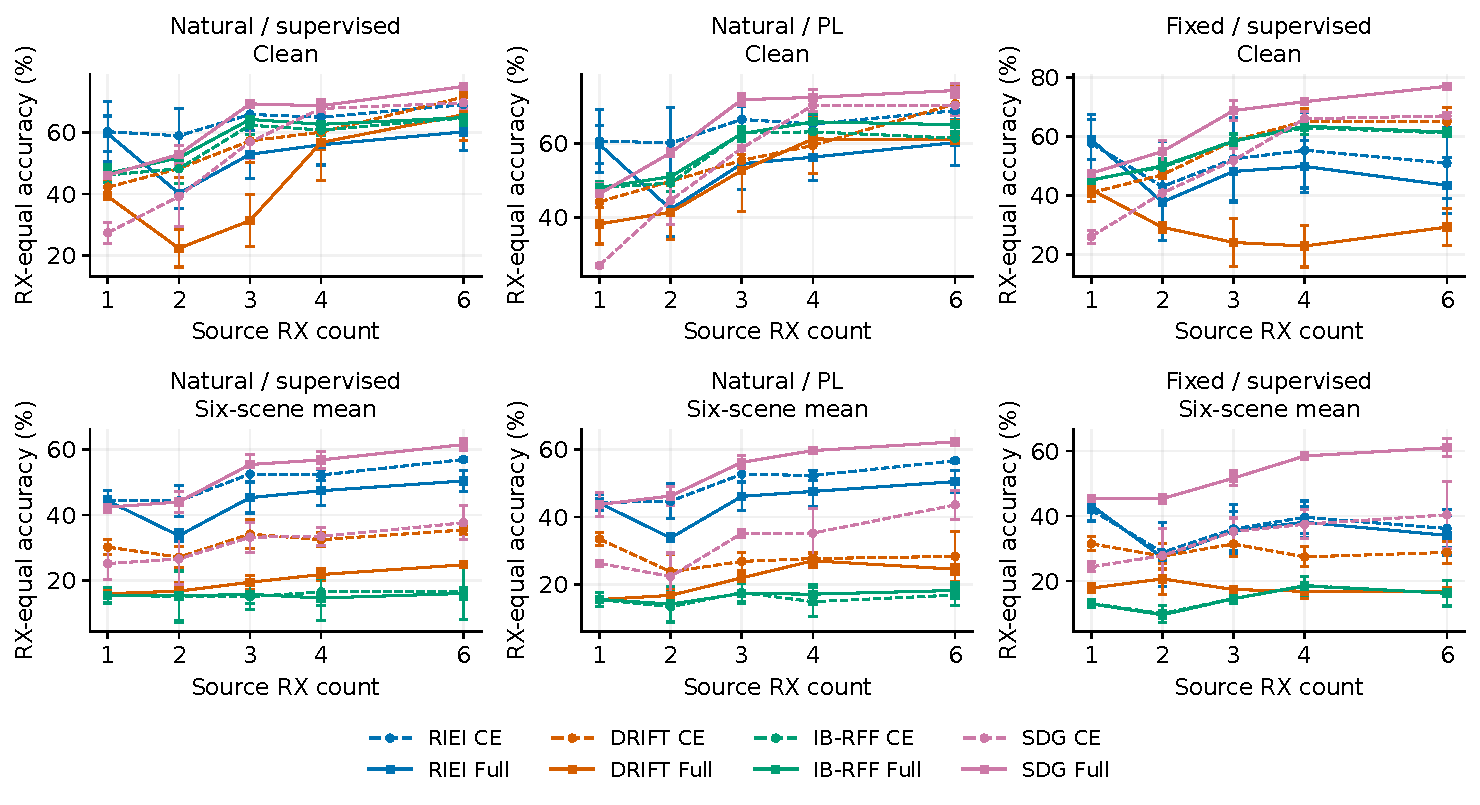
\includegraphics[width=\textwidth]{images/sourcecount/sourcecount_accuracy_overview.pdf}
\caption{Completed external source-count accuracy. Columns separate natural supervision, natural ordinary PL, and fixed-L/V supervision; rows show clean and six-practical-scene means. Points are means of three seeds with sample-SD bars. Dashed CE and solid Full use matched data and augmentation within method; source prefixes and target RX are fixed.}
\label{fig:sourcecount-accuracy}
\end{figure*}

Natural budgets increase labeled, unlabeled and validation counts with $m$, so their curves do not isolate receiver diversity. Fixed supervision uses $|L|=1080$ and $|V|=5400$ for all $m$, with U hidden and unused. It controls annotations and maximum method-specific schedules; IB-RFF source early stopping still changes realized epochs/updates, which are reported per row. Table~\ref{tab:sourcecount-m6} gives the predetermined six-source endpoint. The full per-scene curves, including all negative paired differences, accompany the export.

\begin{table*}[t]
\centering\footnotesize
\caption{Six-source endpoint, RX-equal Accuracy in percent (mean$\pm$sample SD, three seeds). Each Clean/Sat pair denotes clean and the within-seed six-scene mean. All columns share the same six target RX; they are not the seven-target F0 contract.}
\label{tab:sourcecount-m6}
\begin{tabular}{llrrrrrr}
\toprule
Method & Version & \multicolumn{2}{c}{Natural supervised} & \multicolumn{2}{c}{Natural PL} & \multicolumn{2}{c}{Fixed L/V supervised}\\
 & & Clean & Sat & Clean & Sat & Clean & Sat\\
\midrule
RIEI & CE & $69.15\pm0.29$ & $56.89\pm0.49$ & $68.97\pm0.34$ & $56.66\pm0.43$ & $50.92\pm12.01$ & $36.14\pm5.90$\\
RIEI & Full & $60.27\pm6.09$ & $50.35\pm3.25$ & $60.29\pm6.14$ & $50.45\pm3.34$ & $43.45\pm9.52$ & $34.03\pm6.25$\\
DRIFT & CE & $71.62\pm1.45$ & $35.40\pm1.31$ & $70.79\pm4.61$ & $28.28\pm7.50$ & $65.09\pm4.74$ & $28.79\pm3.43$\\
DRIFT & Full & $65.84\pm8.33$ & $24.76\pm0.48$ & $61.00\pm1.23$ & $24.46\pm1.42$ & $29.30\pm6.17$ & $16.83\pm0.39$\\
IB-RFF & CE & $64.82\pm1.98$ & $16.53\pm8.32$ & $61.47\pm1.78$ & $16.83\pm3.02$ & $61.24\pm1.22$ & $16.14\pm4.06$\\
IB-RFF & Full & $64.90\pm2.87$ & $16.02\pm1.80$ & $65.14\pm2.80$ & $18.17\pm2.48$ & $61.51\pm0.95$ & $16.22\pm3.91$\\
SDG & CE & $69.72\pm1.93$ & $37.57\pm5.16$ & $70.44\pm2.82$ & $43.58\pm4.32$ & $67.05\pm1.13$ & $40.38\pm10.26$\\
SDG & Full & $75.05\pm0.97$ & $61.45\pm1.83$ & $74.41\pm1.93$ & $62.25\pm0.96$ & $77.10\pm0.94$ & $61.08\pm2.79$\\
\bottomrule
\end{tabular}
\end{table*}

\subsubsection{Mechanism Gains and Negative Controls}
Figure~\ref{fig:sourcecount-dg} reports same-seed Full-minus-own-CE differences. Across the 120 prespecified clean/six-scene method--regime--count mean contrasts, 67 are nonpositive. These correlated descriptive contrasts are not 120 independent hypothesis tests. Thus this benchmark does not support a claim that native DG mechanisms universally improve on their own backbones. For example, natural-supervised RIEI at six sources gives $69.149\pm0.294\%$ clean and $56.893\pm0.495\%$ six-scene accuracy with CE, versus $60.269\pm6.091\%$ and $50.350\pm3.254\%$ with Full. Conversely, SDG Full at the fixed six-source endpoint gives $77.096\pm0.941\%$ clean and $61.080\pm2.794\%$ six-scene accuracy. This comparison retains each method's declared objective/view recipe and all observed seed variation; no branch is discarded after seeing target results.

\begin{figure*}[t]
\centering
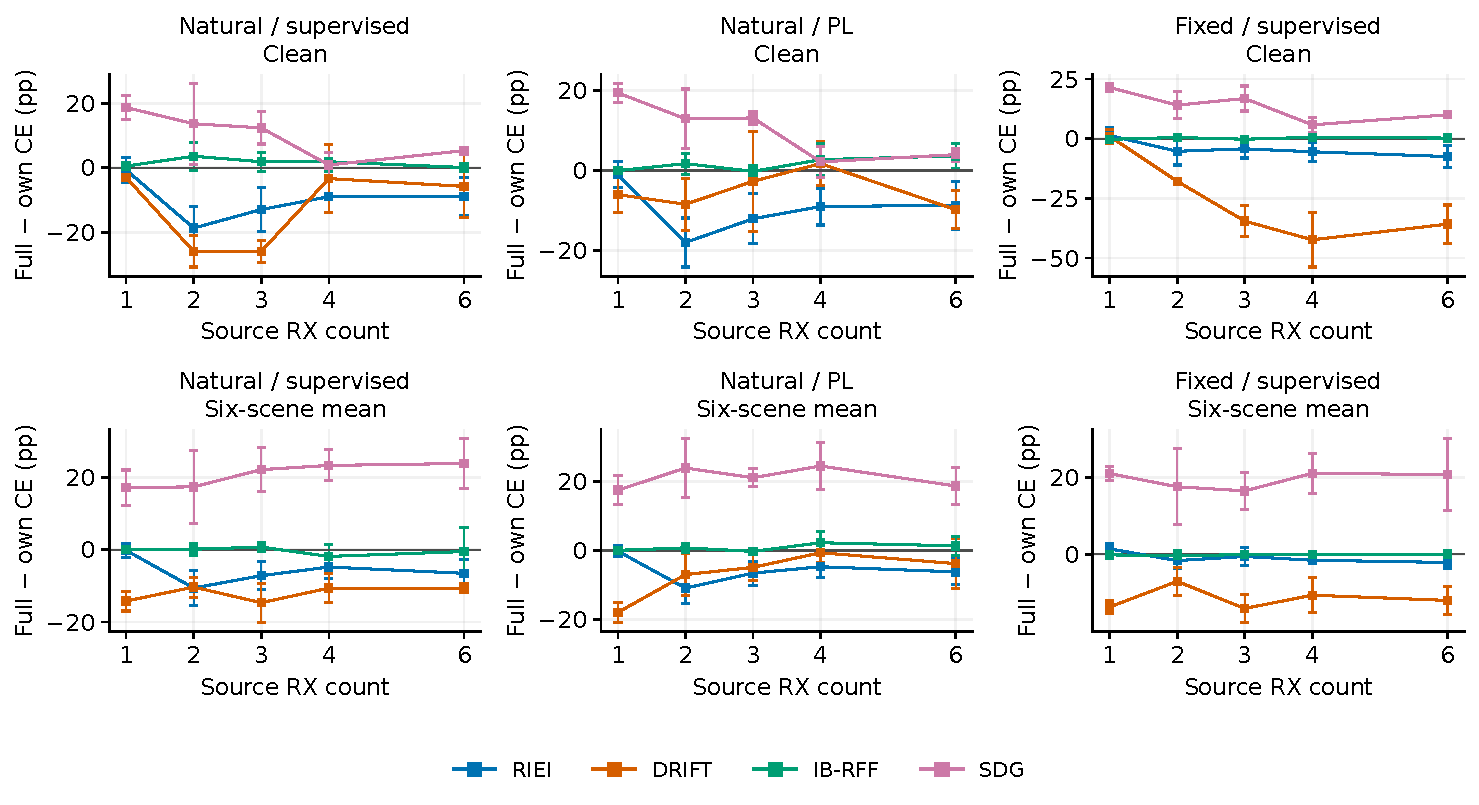
\includegraphics[width=\textwidth]{images/sourcecount/sourcecount_dg_overview.pdf}
\caption{Full-minus-own-CE gains in percentage points under the same conditions as Fig.~\ref{fig:sourcecount-accuracy}. Bars are sample SD of three paired seed differences. The zero line and all negative gains remain visible; a single source provides only one physical receiver domain.}
\label{fig:sourcecount-dg}
\end{figure*}

\subsubsection{Ordinary PL and Realized Training Cost}
PL and satellite concatenation coexist in all 120 natural-PL models. Figure~\ref{fig:sourcecount-pl} reports PL-minus-supervised changes at fixed method, count and seed. All 30 RIEI PL models accept no pseudo labels during training. Their change from supervision cannot be attributed to accepted pseudo-label gradients; joint U forwards can still change batch-normalization and stochastic trajectories. The row-level export reports total and selected-checkpoint U exposure/acceptance, labeled/satellite exposure, realized epochs, batch/optimizer updates, and source-freeze epoch. PL does not consistently improve every setting, and the curves are not forced to be monotonic.

\begin{figure*}[t]
\centering
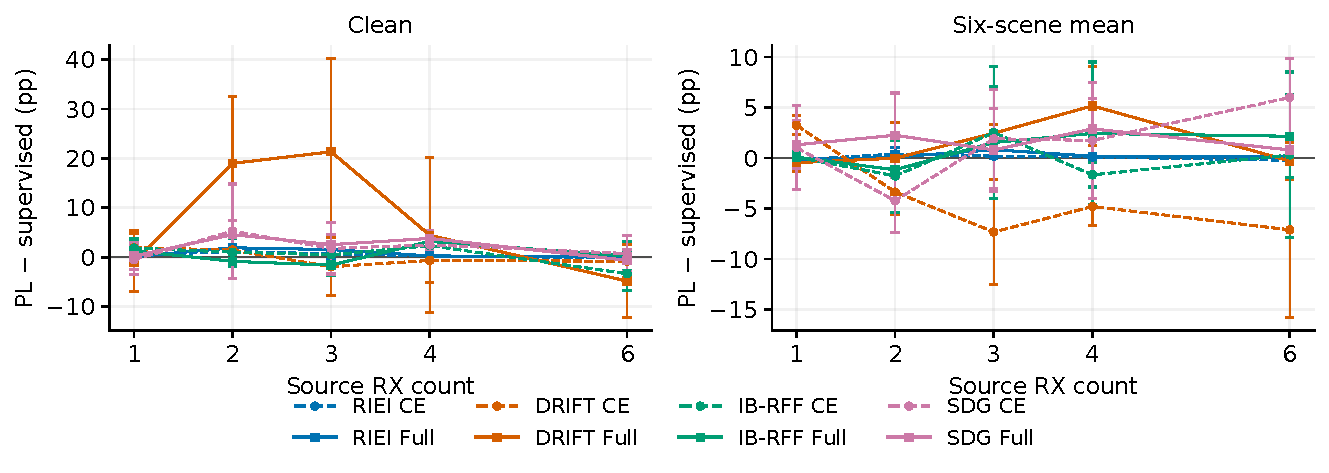
\includegraphics[width=\textwidth]{images/sourcecount/sourcecount_pl_gain_overview.pdf}
\caption{Ordinary PL-minus-supervised paired gains for clean and six-scene mean accuracy. Each Full/CE pair retains the same default satellite concatenation; the PL threshold is 0.95, weight one, and U/L exposure ratio one. Bars are sample SD over three paired model seeds.}
\label{fig:sourcecount-pl}
\end{figure*}

RIEI and DRIFT each train for 100 epochs, and SDG for 200; realized IB-RFF totals range from 31 to 112 epochs over its two source-stopped stages. The sum of measured per-worker source-training elapsed time is 43.236 hours. This is neither exclusive-device GPU compute time nor the experiment's wall-clock makespan; sharing, prediction, scoring, waiting and audit costs are distinct. All m/scene metric tables and ten vector figures with per-scene panels are included in the export. Results are conditional on one predetermined nested RX chain, the fixed six-target engineering benchmark, and the declared budgets. They do not establish a universal receiver-count law or independent in-orbit validation. The PAMF T1/DURA source-count, contract and mechanism matrices continue separately; their pending matched results are not inferred from the completed F0 or external curves.
